\section{ Trigger corrections }

\slide{Effect of new $\eta-\phi$ muon trigger corrections}
{
\centering
\alt<1,3>{\purple{Old} corrections in $\eta-p_{T}$ only}{\purple{New} corrections in $\eta-p_{T}$ x $\eta-phi$}

\colb[T]
\column{.5\textwidth}
\centering
Muon $\Wminus$ \alt<1,2>{$eta$}{$phi$} \\
\includegraphics[width=1.0\textwidth]<1>{dates/20121119/figures/trig/old_eta_NEG.pdf}
\includegraphics[width=1.0\textwidth]<2>{dates/20121119/figures/trig/new_eta_NEG.pdf}
\includegraphics[width=1.0\textwidth]<3>{dates/20121119/figures/trig/old_phi_NEG.pdf}
\includegraphics[width=1.0\textwidth]<4>{dates/20121119/figures/trig/new_phi_NEG.pdf}

\column{.5\textwidth}
\centering
Muon $\Wplus$ \alt<1,2>{$eta$}{$phi$} \\
\includegraphics[width=1.0\textwidth]<1>{dates/20121119/figures/trig/old_eta_POS.pdf}
\includegraphics[width=1.0\textwidth]<2>{dates/20121119/figures/trig/new_eta_POS.pdf}
\includegraphics[width=1.0\textwidth]<3>{dates/20121119/figures/trig/old_phi_POS.pdf}
\includegraphics[width=1.0\textwidth]<4>{dates/20121119/figures/trig/new_phi_POS.pdf}
\cole
\only<1>{\footnotesize{Positive-negative $\eta$ appears asymmetric: even ignoring choppiness, A-side seems higher. }}
\only<2>{\footnotesize{No obvious improvement. In fact, the \red{last eta bin} seems to have gotten worse.}}
\only<3>{\footnotesize{A lot of structure in $\phi$. The structure is mostly charge-symmetric. }}
\only<4>{\footnotesize{But adding the new $\phi$ corrections \red{does not seem to make it better}. Bug? }}
}

\slide{Plotting event trigger weights in signal MC }
{
\centering
\alt<1,2>{Old corrections in $\eta-p_{T}$ only}{New corrections in $\eta-p_{T}$ x $\eta-phi$}
\colb[T]
\column{.5\textwidth}
\centering
Muon $\Wminus$ trigger weight \\
\includegraphics[width=0.8\textwidth]<1>{dates/20121119/figures/trig/old_trigw_NEG.pdf}
\includegraphics[width=0.8\textwidth]<2>{dates/20121119/figures/trig/new_trigw_NEG.pdf}

\column{.5\textwidth}
\centering
Muon $\Wplus$ trigger weight \\
\includegraphics[width=0.9\textwidth]<1>{dates/20121119/figures/trig/old_trigw_POS.pdf}
\includegraphics[width=0.9\textwidth]<2>{dates/20121119/figures/trig/new_trigw_POS.pdf}
\cole

\only<1>{\footnotesize{``Choppiness'' is due to binned nature of the trigger scale factors. }}
\only<2>{\footnotesize{Note a higher RMS and more smoothness due to large phase space of corrections.}}
}



%===========================================
%  Z plots
%===========================================
\section{ Z plots }

\slide{Muon mass scale is based on $\Zboson$ events}
{
\centering
Ratio plot is flat around Z mass peak. Deviations away from the peak are due to BG modeling.
\newline
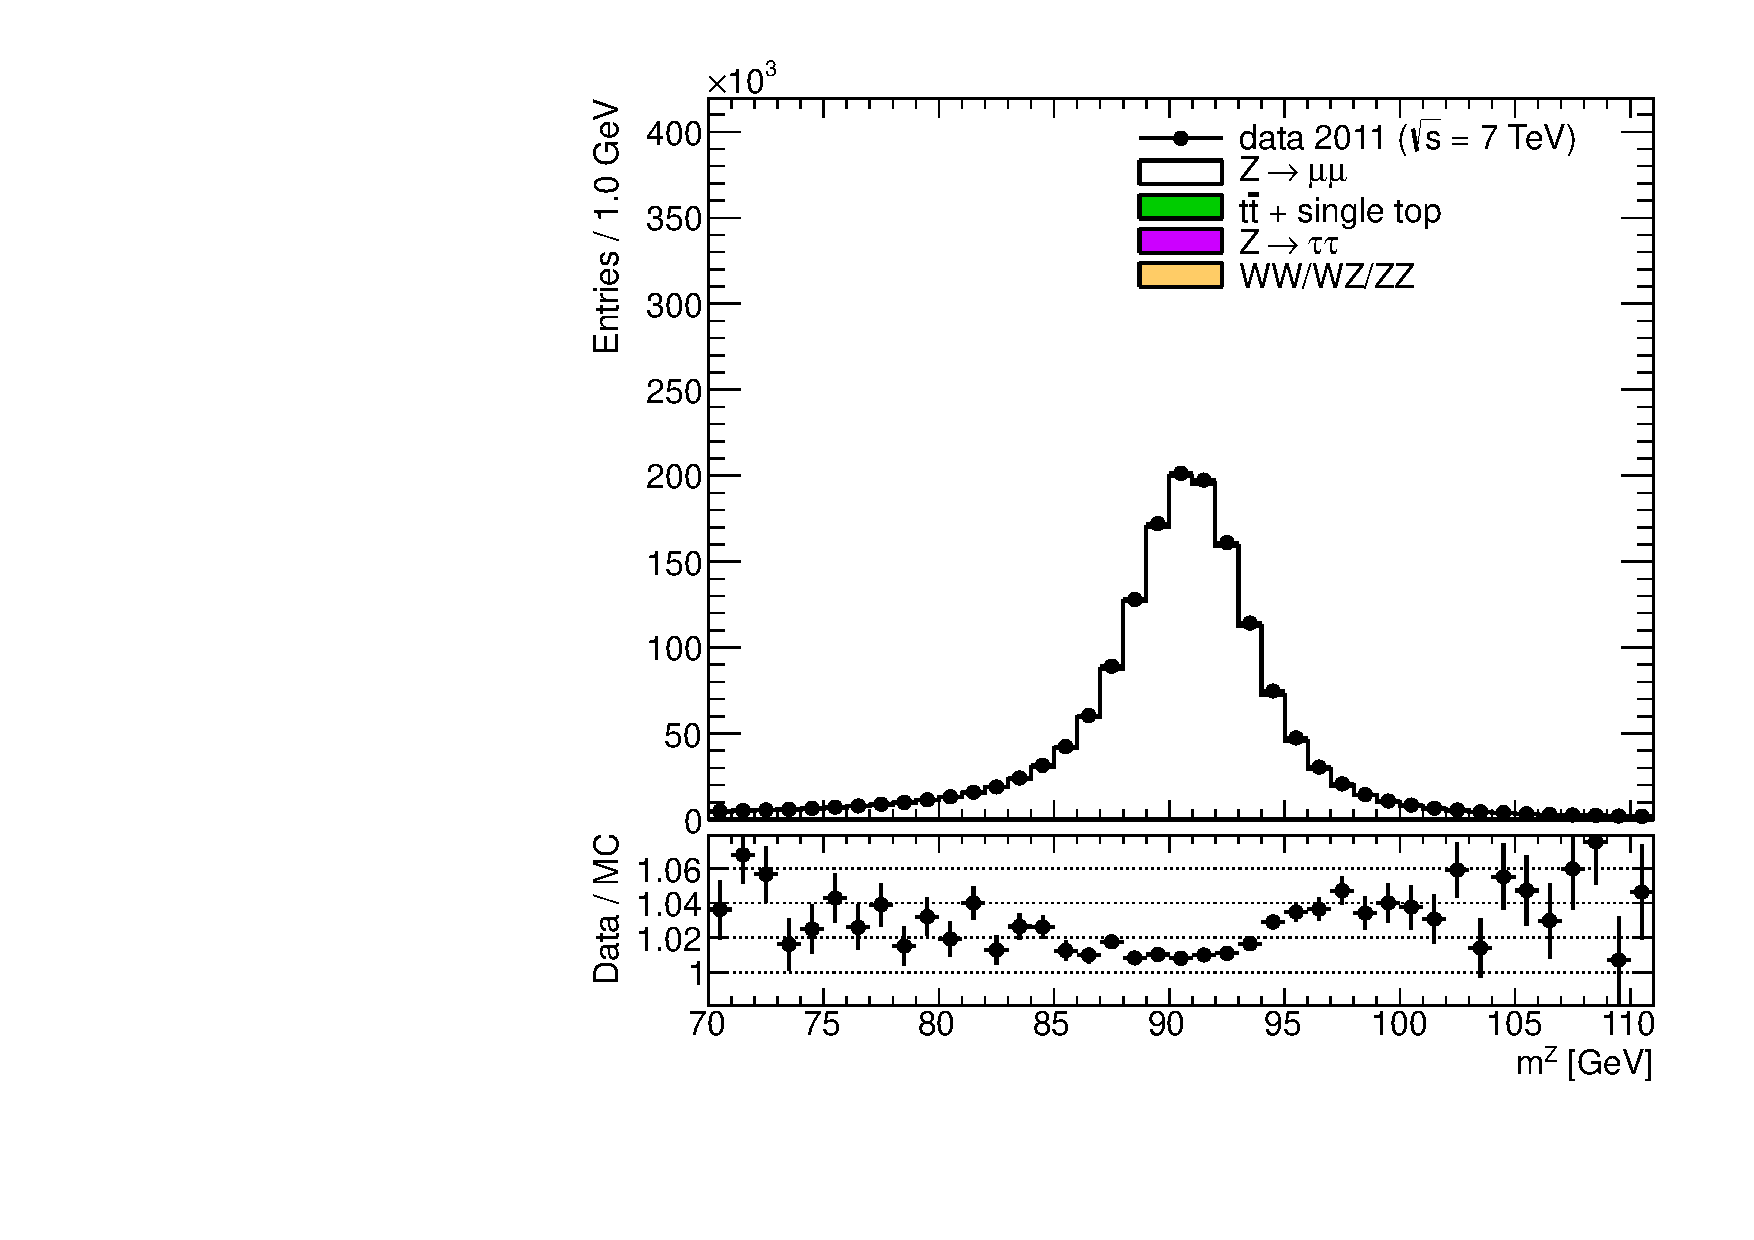
\includegraphics[height=0.9\textheight]{dates/20121119/figures/zplots/zm_nomatch.pdf}
}

\slide{$\eta$ of muons in $\Zboson$ events}
{
\centering
Ratio plot is zoomed-in. No extra large fluctuations.
\newline
\colb[T]
\column{.5\textwidth}
\centering
$\mu^-$ $\eta$ \\
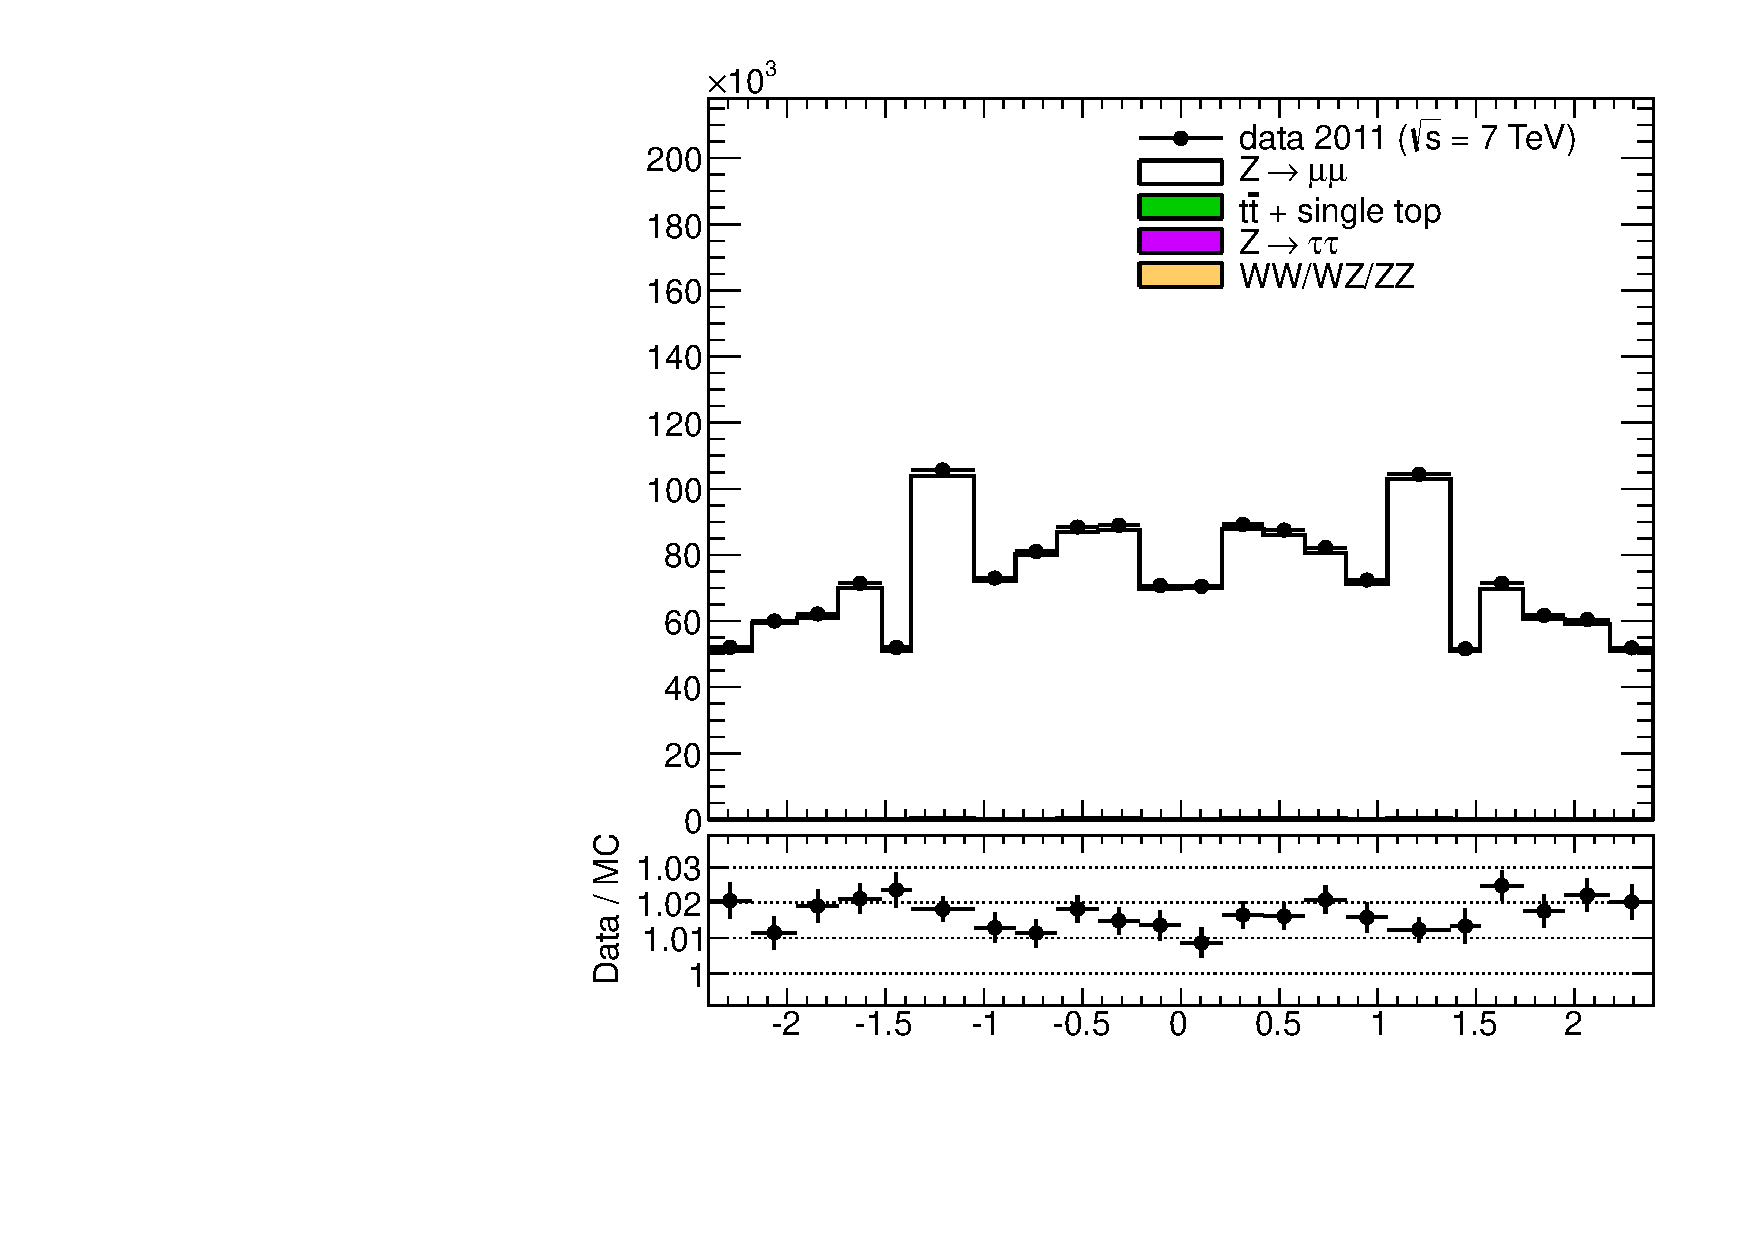
\includegraphics[width=1.0\textwidth]{dates/20121119/figures/zplots/lN_eta_nomatch.pdf}

\column{.5\textwidth}
\centering
$\mu^+$ $\eta$ \\
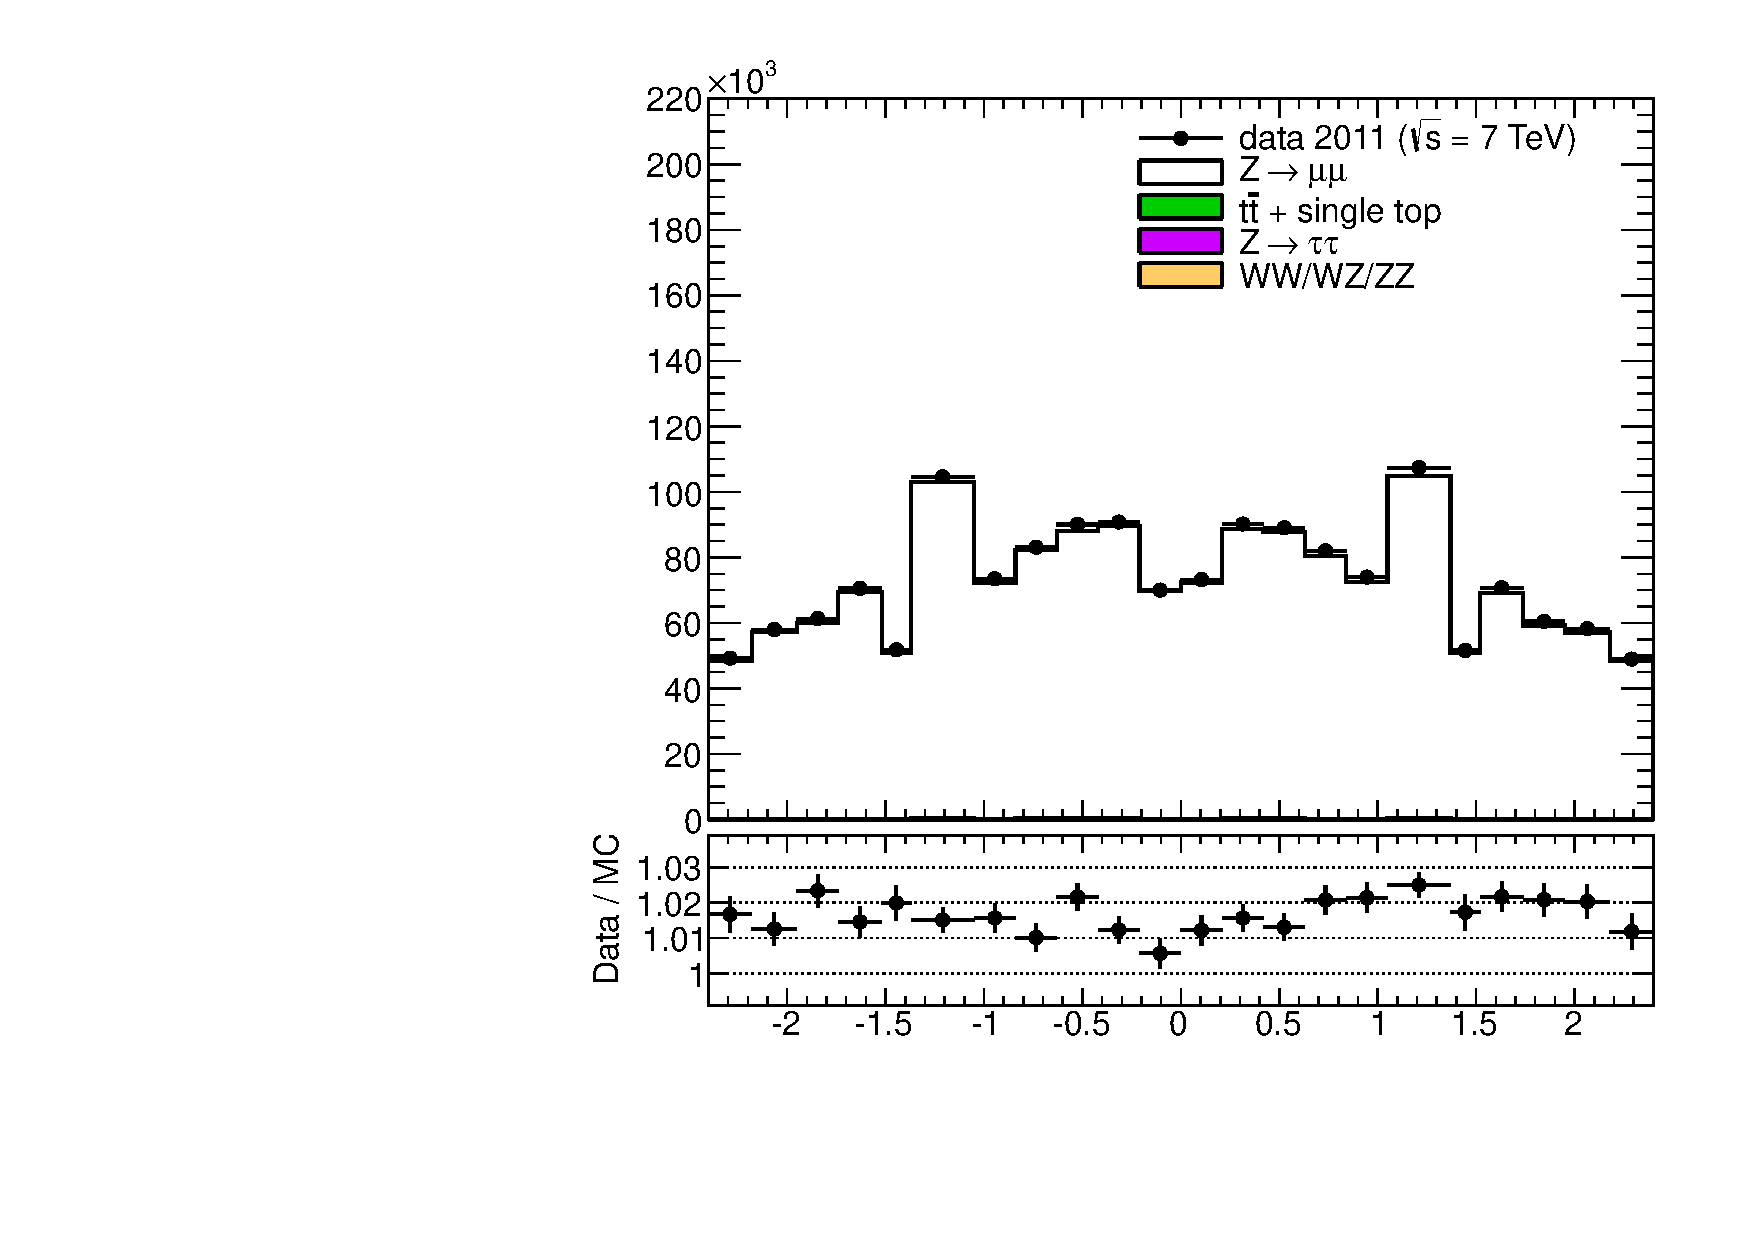
\includegraphics[width=1.0\textwidth]{dates/20121119/figures/zplots/lP_eta_nomatch.pdf}
\cole
}

\slide{$\phi$ of muons in $\Zboson$ events (no extra $\phi$ correction)}
{
\centering
Structure in $\phi$ is mostly charge-symmetric and different from $\Wboson$
\newline
\colb[T]
\column{.5\textwidth}
\centering
$\mu^-$ $\phi$ \\
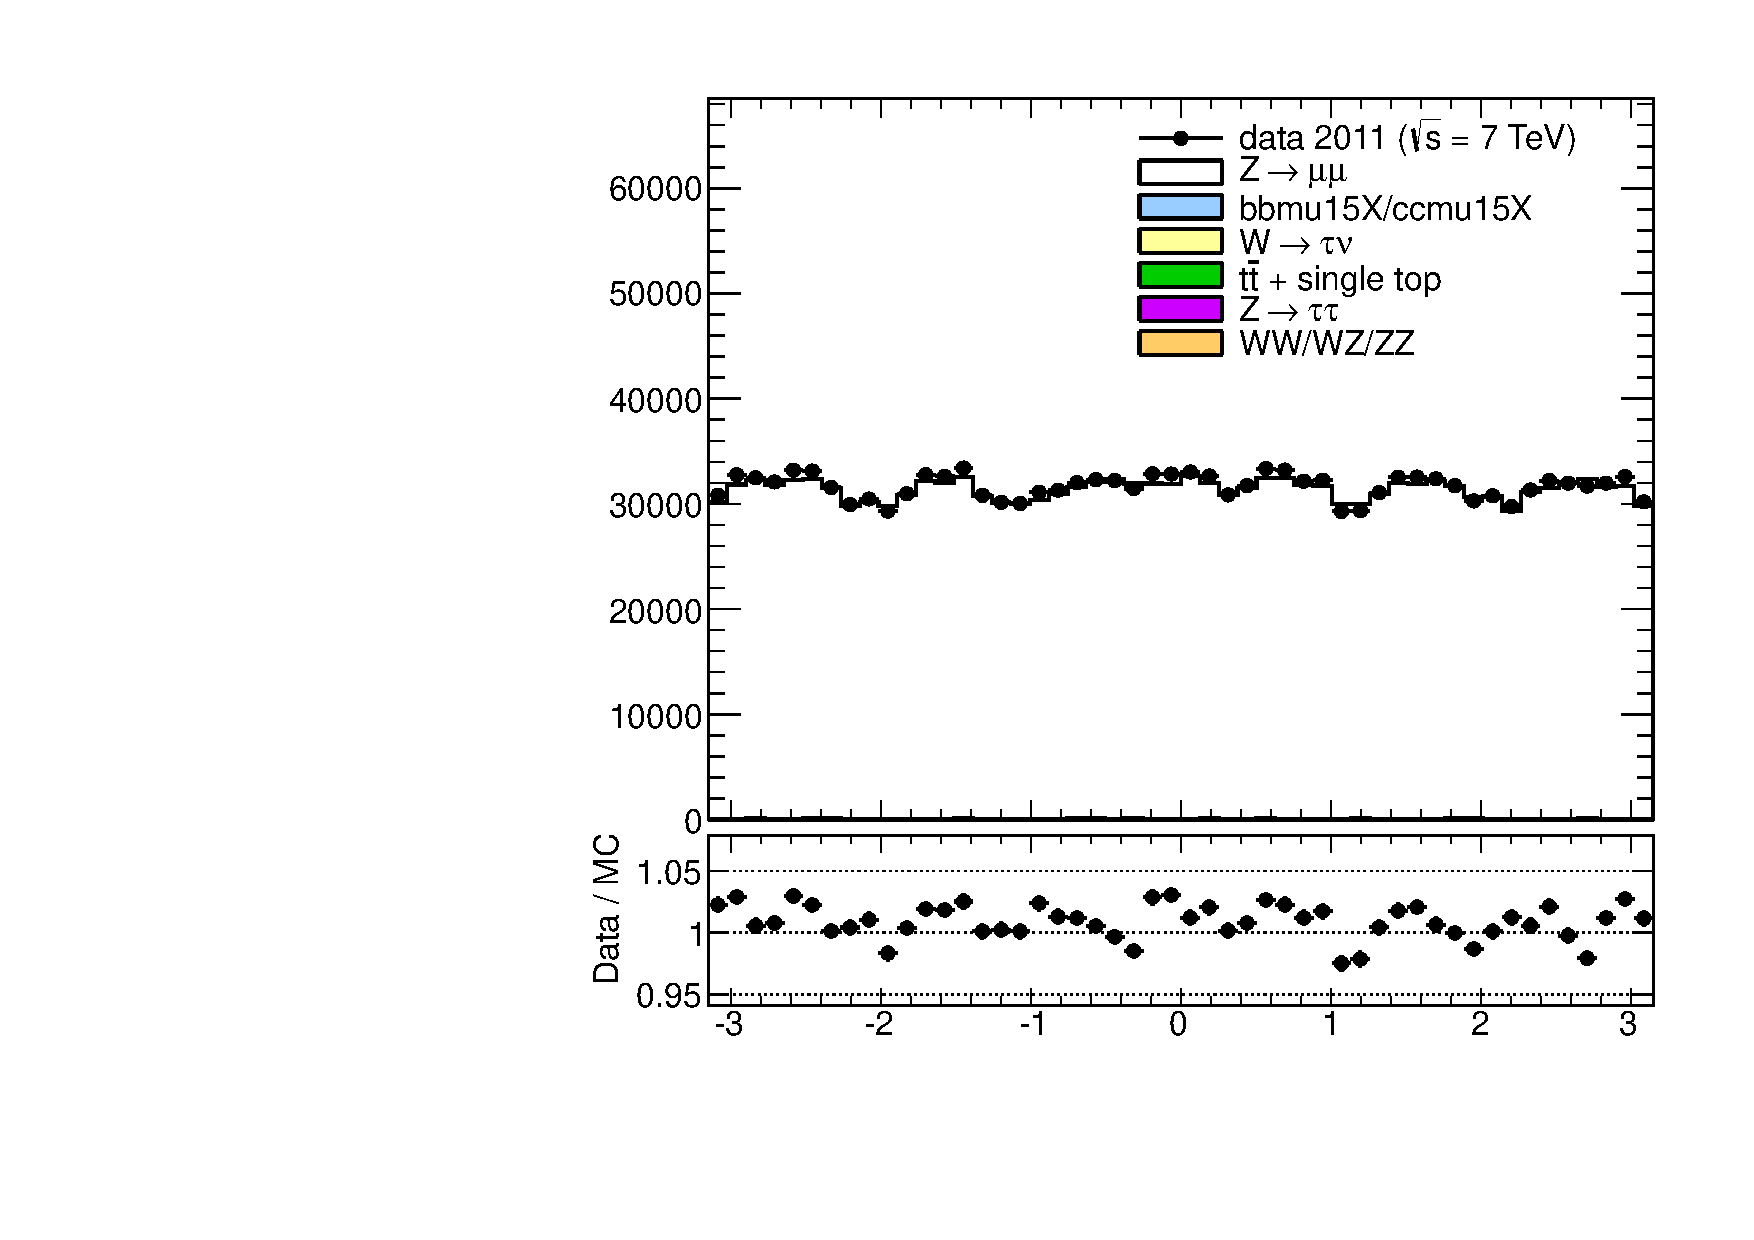
\includegraphics[width=1.0\textwidth]{dates/20121119/figures/zplots/lN_phi_nomatch.pdf}

\column{.5\textwidth}
\centering
$\mu^+$ $\phi$ \\
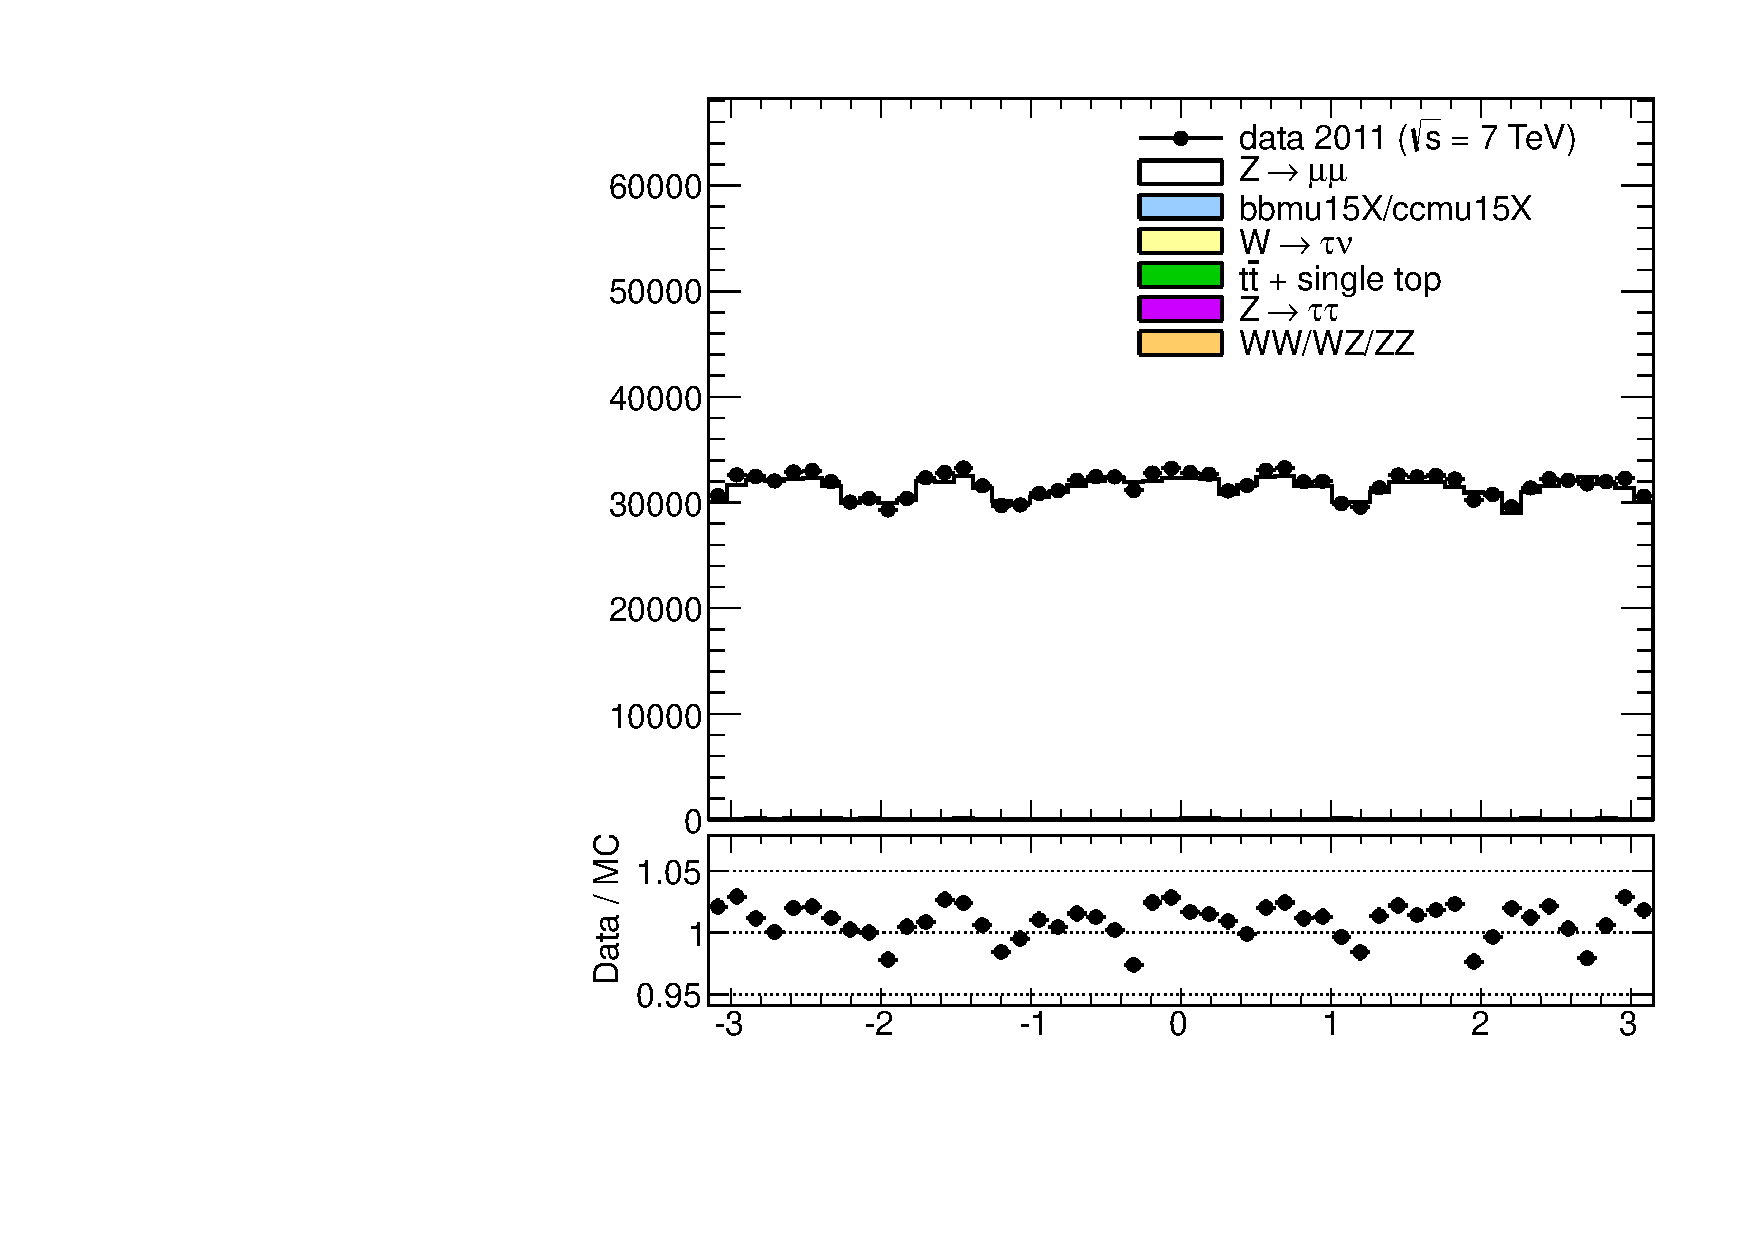
\includegraphics[width=1.0\textwidth]{dates/20121119/figures/zplots/lP_phi_nomatch.pdf}
\cole
}
